\documentclass[times]{elsarticle}

\usepackage[dvipsnames]{xcolor}
\usepackage{amsmath}
\usepackage{amsfonts}
\usepackage{amssymb}
\usepackage{lineno}
\usepackage{enumerate}
\usepackage{times}
\usepackage{subcaption}
\usepackage{graphicx,psfrag}
\usepackage{pgfplotstable}
\usepackage[skip=0pt]{caption}

\newcommand\solidrule[1][0.25cm]{\rule[0.5ex]{#1}{1pt}}
\newcommand\dashedrule{\mbox{%
  \solidrule[2mm]\hspace{2mm}\solidrule[2mm]}}

\newcommand{\dotrule}[1][4mm]{%
	\parbox{#1}{\dotfill}} 

\makeatletter
\newcommand \Dotfill {\leavevmode \cleaders \hb@xt@ .22em{\hss .\hss }\hfill \kern \z@}
\makeatother
 
\newcommand{\Dotrule}[1]{%
   \parbox{#1}{\Dotfill}} 

  \DeclareRobustCommand{\squaret}[1]{\tikz{\draw[#1,thick] (0,0) rectangle (0.2cm,0.2cm);}}
  \DeclareRobustCommand{\circlet}[1]{\tikz{\draw[#1,thick] (0,0) circle [radius=0.1cm];}}
  \DeclareRobustCommand{\trianglet}[1]{\tikz{\draw[#1,thick] (0,0) --
  		(0.25cm,0) -- (0.125cm,0.25cm) -- (0,0);}}
  \DeclareRobustCommand{\crosst}[1]{\tikz{\draw[#1,thick] (0cm,0cm) --
  		(0.1cm,0.1cm) -- (0cm,0.2cm) -- (0.1cm,0.1cm) -- (0.2cm,0.2cm) -- (0.1cm,0.1cm)-- (0.2cm,0cm);}}
  \DeclareRobustCommand{\diamondt}[1]{\tikz{\draw[#1,thick] (0,0) --(0.1cm,0.15cm) -- (0.2cm,0cm) -- (0.1cm,-0.15cm) -- (0,0)  ;}}
  \DeclareRobustCommand{\squareF}[1]{\tikz{\filldraw[#1,fill opacity= 0.3] (0,0) rectangle (0.2cm,0.2cm);}}

  \newcommand\T{\rule{0pt}{5ex }}       % Top table strut
  \newcommand\B{\rule[-4ex]{0pt}{4ex }} % Bottom table strut
  
  \newcommand\TM{\rule{0pt}{2.8ex }}       % Top matrix strut
  \newcommand\BM{\rule[-2ex]{0pt}{2ex }} % Bottom matrix strut
  \newcommand{\matr}[1]{\mathbf{#1}}
  \newcommand{\vecn}[1]{\boldsymbol{#1}}

\begin{document}

\title{Solving the fully non-linear weakly dispersive Serre equations for flows over dry beds.}

\author[ANU]{J.P.A.~Pitt\corref{cor1}}
\ead{jordan.pitt@anu.edu.au }
\author[ANU]{C.~Zoppou}
\ead{christopher.zoppou@anu.edu.au}
\author[ANU]{S.G.~Roberts}
\ead{stephen.roberts@anu.edu.au}

\cortext[cor1]{Corresponding author}
\address[ANU]{Mathematical Sciences Institute, Australian National University, Canberra, ACT 0200, Australia}
 
 
%To do:
% Abstract
%Spelling
%Bibliography
%consistent equations
%Synolakis plot t = 0 
 \begin{abstract}
 	We describe a numerical method for solving the Serre equations that can model flows over dry varying beds. The method solves the Serre equations in conservation law form with a finite volume method. Where a finite element method is used to solve the auxiliary elliptic equation for the depth-averaged horizontal velocity. The numerical method is validated against the lake at rest analytic solution, demonstrating that it is well-balanced. The method is further validated and its convergence rate established using forced solutions containing the wetting and drying of varying beds. The use of forced solutions extends the validations performed for previous Serre equation solvers for flows over dry varying beds. Finally, the method is validated against experimental results for the run-up of a solitary wave on a sloped beach.

 \end{abstract}	
 
  \begin{keyword}
  	Serre equations\sep dry bed
  \end{keyword}
  
 \maketitle
\linenumbers
%--------------------------------------------------------------------------------
\section{Introduction} \label{intro} 

%Other papers:
%Fillipine : 
%\cite{Li-2014-169} - do dry beds as well, no convergence test though, no wave breaking
%\cite{Filippini-etal-2016-381} - do dry beds as well, but with wavebreaking, revert to SWWE, no convergence test though (splitting)
%\cite{Tissier} run up with wave breaking, revert to SWWE (splitting)
%\cite{DoCarmo-2019-125} run up with wave breaking, revert to SWWE (splitting)

Dispersion is an important attribute of waves in intermediate water depths; where the water depth is not much larger than the wavelengths of the waves. Our understanding of the effect of dispersion on water surface profiles is continually improving \cite{Pitt-2018-61}. However, what is not well understood is the behaviour of these waves as they approach and then inundate the coastline. 

There is a family of dispersive wave equations that can be used to model the behaviour of dispersive waves as they inundate a dry bed. The Serre equations \cite{Serre-F-1953-857} are important among the family of dispersive wave equations, as they do not make assumptions about the wave amplitude and so are fully non-linear. For this reason they are considered the most appropriate model of dispersive waves as they approach and then inundate the coastline \cite{Bonneton-Lannes-2009-16601}.

Previous work has resulted in the development of numerical methods for Serre equations that can model flows over dry beds \cite{Tissier-2011,Li-2014-169,Filippini-etal-2016-381,DoCarmo-2019-125}. The most popular approach to solve the Serre equations in the literature is to split the Serre equations into their hyperbolic part given by the Shallow Water Wave Equations (SWWE) and their dispersive part \cite{Tissier-2011,Filippini-etal-2016-381,DoCarmo-2019-125}. Additionally, these splitting schemes employ modifications to simulate wave-breaking; where only the hyperbolic part is solved when some local wave breaking criteria is met. 

Currently, there are no known analytic solutions to the Serre equations that include varying bathymetry and the wetting and drying of the bed. Hence, numerical methods in the literature have relied on experimental results to demonstrate their capability in these situations \cite{Tissier-2011,Li-2014-169,Filippini-etal-2016-381,DoCarmo-2019-125}. We extend these validation results in the literature by using forced solutions of the Serre equations. Forced solutions allow the ability of the method to accurately solve problems with varying bathymetry and the wetting and drying of the bed to be tested without analytic solutions. Furthermore, they permit a convergence analysis to demonstrate the order of accuracy of the method in these situations. 

This paper also builds upon the work of \citet{Zoppou-etal-2017} on the Finite Difference Volume Methods (FDVM) for the Serre equations, describing a Finite Element Volume Method (FEVM) extension of the FDVM. In the FEVM a Finite Element Method is used to solve the auxiliary elliptic equations instead of the finite difference methods used by the FDVM, leading to a more robust numerical method.

The Serre equations and their conservation properties will now be presented. Followed by a description of the FEVM. The numerical scheme will be validated against the lake at rest analytic solution, demonstrating that it is well-balanced. The method will then be validated for the wetting and drying of the bed using forced solutions to the Serre equations. Finally, the numerical method is validated against the experimental results of \citet{Synolakis-1987-523} for the run-up of a solitary wave on a dry linear beach.

%--------------------------------------------------------------------------------
\section{Serre Equations}
The Serre equations \cite{Seabra-Santos-etal-1987-117} are a system of partial differential equations that describe the free-surface waves of fluids whose motion is dominated by gravitational forces. The primitive variables of the Serre equations are the height of the free-surface $h(x,t)$ above the bed $b(x)$ and the depth-averaged horizontal velocity of a column of water $u(x,t)$. These variables are shown in Figure \ref{fig:SerreModel}. The absolute location of the free surface is given by $w(x,t) = h(x,t) + b(x)$.
\begin{figure}
	\centering
	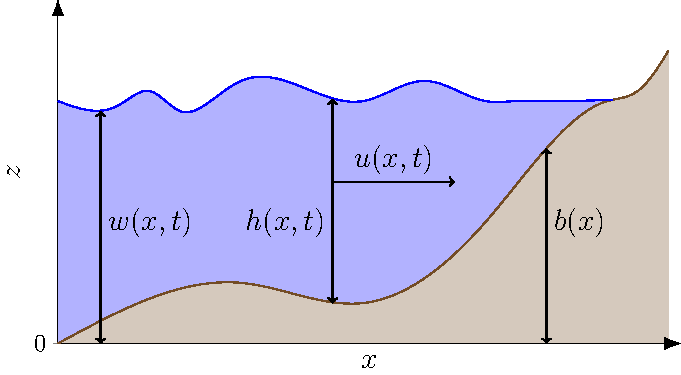
\includegraphics[width=0.55\textwidth]{./Figures/Diagrams/Watermodel/SerreModel.pdf}
	\caption{Diagram demonstrating a free surface flow (\squareF{blue}) over a bed (\squareF{brown!80!black}) where $w(x,t)$ is the absolute location of the free surface, $h(x,t)$ is the height of a column of fluid, $u(x,t)$ is the depth-averaged horizontal velocity of a column of fluid and $b(x)$ is the stationary bed profile.}
	\label{fig:SerreModel}
\end{figure}

The Serre equations can be written in conservation law form with a source term \cite{Zoppou-etal-2017} like so
\begin{subequations}
	\label{eqn:FullSerreCon}
	\begin{align}
	& \frac{\partial h}{\partial t} + \dfrac{\partial (uh)}{\partial x} = 0 ,\label{eqn:FullSerreConMass}  \\ \nonumber \\
	\begin{split}
	\label{eqn:Serreconsconmom}
	\frac{\partial G}{\partial t}  + \frac{\partial}{\partial x} \left( {u} G + \frac{gh^2}{2} - \frac{2h^3}{3} \left[\frac{\partial {u}}{\partial x}\right]^2 + h^2 {u}\frac{\partial {u}}{\partial x}\frac{\partial b}{\partial x} \right) \\ \\ +  \underbrace{\frac{uh^2}{2} \frac{\partial {u}}{\partial x} \frac{\partial^2 b}{\partial x^2}  - h {u}^2\frac{\partial b}{\partial x}\frac{\partial^2 b}{\partial x^2} + gh\frac{\partial b}{\partial x} } _{\text{source term}} = 0
	\end{split}
	\end{align}
\end{subequations}
with the conserved quantity
\begin{equation}
\label{defn:SerreEqnConservedQuantity1}
G =  {u}h \left(1 + \frac{\partial h}{\partial x}\frac{\partial b}{\partial x} + \frac{h}{2}\frac{\partial^2 b}{\partial x^2} + \left[\frac{\partial b}{\partial x}\right]^2 \right) - \frac{\partial}{\partial x}\left(\frac{h^3}{3}  \frac{\partial {u}}{\partial x}\right).
\end{equation}

\subsection{Conservation Properties}
Since the Serre equations can be written in conservation law form for $h$ and $G$ these quantities should be conserved in a closed system. Where conservation of a quantity $q$ means that the total amount of $q$ in a system occurring on the interval $[a,b]$ at time $t$
\begin{equation*}
\mathcal{C}_q(t) = \int_{a}^{b} q(x,t)\, dx
\end{equation*}
remains constant for all $t$. Additionally, the Serre equations conserve the momentum $uh$ and the energy
\begin{equation*}
\mathcal{H}(x,t) = \frac{1}{2} \left( gh\left(h + 2b\right) + hu^2  + \frac{h^3}{3} \left[\frac{\partial u}{\partial x}\right]^2 + u^2h\left[\frac{\partial b}{\partial x}\right]^2 - uh^2 \frac{\partial u}{\partial x} \frac{\partial b}{\partial x}  \right).
\label{eqn:Hamildef}
\end{equation*}
The conservation of $uh$ is a result of integrating the evolution of momentum equation for Serre equations \cite{Zoppou-etal-2017}. An equivalent set of equations in one-dimension was produced by \citet{Green-Naghdi-1976-237} through conservation of the energy $\mathcal{H}$, and hence the Serre equations conserve $\mathcal{H}$. With $\mathcal{H}$ being a sum of the gravitational potential and kinetic energy throughout the depth of water. 

%--------------------------------------------------------------------------------
\section{Method}
To numerically approximate the Serre equations in conservation law form \eqref{eqn:FullSerreCon} the domain is partitioned into $m$ cells $\left[x_{j-1/2},x_{j+1/2}\right]$ of uniform length $\Delta x$. While time is discretised into time levels $t^n$ separated by a constant duration $\Delta t$.

Since the Serre equations are in conservation law form
\begin{equation*}
\frac{\partial \vecn{Q} }{\partial t} + \frac{\partial F(\vecn{Q} )}{x} + S(\vecn{Q} ) = 0
\end{equation*}
with the conserved quantities $\vecn{Q}  = \left[h \; \; G\right]$ they can be solved using a Finite Volume Method (FVM) with a source term approximation like so
\begin{equation}
\label{eqn:FVMUpdate}
\overline{\vecn{Q} }^{n+1}_j = \overline{\vecn{Q} }^{n}_j - \frac{\Delta t}{\Delta x} \left(F^n_{j+1/2}\left(\vecn{Q} \right) - F^n_{j-1/2}\left(\vecn{Q} \right) \right) + \Delta t S^n_j\left(\vecn{Q} \right)
\end{equation}
which employs first-order forward Euler time integration. Where $\overline{\vecn{Q} }^{n}_j $ is the average of the conserved quantities in the $j^{th}$ cell at time $t^n$. While $F^n_{j+1/2}\left(\vecn{Q} \right)$ and $ F^n_{j-1/2}\left(\vecn{Q} \right)$ are approximations to the flux across the right and left boundaries respectively and $S^n_j\left(\vecn{Q} \right)$ is the approximation to the source terms contribution to the cell from time $t^n$ to $t^{n+1}$. The FVM \eqref{eqn:FVMUpdate} produces a first-order time stepping method, second-order accuracy is achieved using a Strong Stability Preserving Runge-Kutta method \cite{Gottlieb-etal-2003-89} which uses a convex combination of multiple time-steps given by \eqref{eqn:FVMUpdate}.

To approximate the intercell fluxes $F^n_{j+1/2}\left(\vecn{Q} \right)$ and $F^n_{j-1/2}\left(\vecn{Q} \right)$ we use the method of \citet{Kurganov-etal-2001-707}. While the source term is approximated with the well-balancing modifications proposed by \citet{Klein-etal-2004-2050}.

To achieve a second-order accurate method using \eqref{eqn:FVMUpdate} second-order accurate approximations to $h$, $u$, $G$, $\partial u / \partial x$, $\partial b / \partial x$, $\partial^2 b / \partial x^2$ inside a cell are required. The conserved quantities $h$ and $G$ are reconstructed from their cell averages, resulting in a linear approximation to $h$ and $G$ over the cell. While $b$ is reconstructed using a cubic polynomial to ensure that the approximation to $\partial^2 b / \partial x^2$ in the source term \eqref{eqn:FullSerreCon} is second-order accurate. 

The depth-averaged velocity $u$ is obtained by solving \eqref{defn:SerreEqnConservedQuantity1} with a FEM given the reconstructions of $h$, $G$ and $b$ over the cell. Thus all the required approximations are obtained allowing the use of the FVM \eqref{eqn:FVMUpdate} to solve \eqref{eqn:FullSerreCon} as desired.

\subsection{Flux Approximation}
%ddot
We use the method of \citet{Kurganov-etal-2001-707} to calculate the flux across a cell interface. This method was employed because it can handle discontinuities across the cell boundary and only requires an estimate of the maximum and minimum wave speeds, which are known for the Serre equations \cite{Zoppou-etal-2017}.

Only the calculation of the flux term $F^n_{j+1/2}\left(\vecn{Q} \right)$ is demonstrated as the process to calculate the flux term $F^n_{j-1/2}\left(\vecn{Q} \right)$ is identical but involves different cells. For a general quantity $q$ the approximation of the flux term given by \citet{Kurganov-etal-2001-707} is
\begin{equation}\label{eqn:HLL_flux}
F^n_{j+\frac{1}{2}}(q) = \dfrac{a^+_{j+\frac{1}{2}} f\left(q^-_{j+\frac{1}{2}}\right) - a^-_{j+\frac{1}{2}} f\left(q^+_{j+\frac{1}{2}}\right)}{a^+_{j+\frac{1}{2}} - a^-_{j+\frac{1}{2}}}  + \dfrac{a^+_{j+\frac{1}{2}} \, a^-_{j+\frac{1}{2}}}{a^+_{j+\frac{1}{2}} - a^-_{j+\frac{1}{2}}} \left(  q^+_{j+\frac{1}{2}} - q^-_{j+\frac{1}{2}} \right)
\end{equation}

where $a^+_{j+\frac{1}{2}}$ and $a^-_{j+\frac{1}{2}}$ are given by bounds on the wave speed. With all the quantities on the right hand side representing their respective quantities at time $t^n$. Applying the wave speed bounds \cite{Zoppou-etal-2017} we obtain
\begin{subequations}
\begin{align}
a^-_{j+\frac{1}{2}} &= \min\left\lbrace 0\;,\;  u^-_{j + 1/2} - \sqrt{g  {h}^-_{j + 1/2}}  \;,\;u^+_{j + 1/2} - \sqrt{g  {h}^+_{j + 1/2}} \right\rbrace  ,\\
a^+_{j+\frac{1}{2}} &= \max\left\lbrace 0 \;,\;  u^-_{j + 1/2} + \sqrt{g {h}^-_{j + 1/2}}  \;,\;u^+_{j + 1/2} + \sqrt{g  {h}^+_{j + 1/2}} \right\rbrace .
\end{align}
\label{eqn:WaveSpeedBoundsFluxApprox}
\end{subequations}

The flux functions $f(q^-_{j+\frac{1}{2}})$ and $f(q^+_{j+\frac{1}{2}})$ across the cell edge $x_{j+1/2}$ are evaluated using the reconstructed values $q^-_{j+\frac{1}{2}}$ from the $j^{th}$ cell and $q^+_{j+\frac{1}{2}}$ from the $(j+1)^{th}$ cell. For the continuity equation \eqref{eqn:FullSerreConMass} we have
\begin{align}
f\left(h^\pm_{j+\frac{1}{2}}\right) &= u^\pm_{j + 1/2}  {h}^\pm_{j + 1/2}
\label{eqn:FluxMassNum}
\end{align}
and for $G$, \eqref{eqn:Serreconsconmom} we obtain
\begin{align}
f\left(G^\pm_{j+\frac{1}{2}}\right) &=  u^\pm_{j + 1/2} G^\pm_{j + 1/2}  + \frac{g}{2}\left({h}^\pm_{j + 1/2} \right)^2 - \frac{2}{3}\left({h}^\pm_{j + 1/2}\right)^3 \left[\left(\frac{\partial {u}}{\partial x} \right)^\pm_{j + 1/2} \right]^2 \nonumber\\ &+ \left({h}^\pm_{j + 1/2}\right)^2 u^\pm_{j + 1/2} \left(\frac{\partial {u}}{\partial x} \right)^\pm_{j + 1/2} \left(\frac{\partial b}{\partial x} \right)^\pm_{j + 1/2} .
\label{eqn:FluxIrrotNum}
\end{align}

The quantities ${h}^+_{j - 1/2}$, ${h}^-_{j + 1/2}$, $G^+_{j - 1/2}$, $G^-_{j + 1/2}$ and $ \left({\partial {b}}/{\partial x} \right)^\pm_{j + 1/2}$ are given by the reconstructions. While $u^\pm_{j+1/2}$ and $ \left({\partial {u}}/{\partial x} \right)^\pm_{j + 1/2}$ are obtained by the solution of the FEM.

\subsection{Reconstruction}
We reconstruct $h$ and $G$ with piecewise linear functions over a cell from neighbouring cell averages. While $b$ is reconstructed from the nodal values of the neighbouring cells $j-2$, $j-1$, $j+1$ and $j+2$ with a cubic polynomial over those cells. Using a cubic polynomial ensures that the approximation to $\partial^2 b / \partial x^2$ in \eqref{eqn:FullSerreCon} is second-order accurate in cell $j$. The location of the reconstructions for $h$, $G$ and $b$ are given in Figure \ref{fig:ReconLocs}, with their corresponding reconstruction functions being the polynomials that pass through their values at these locations. The bed is reconstructed at the cell edges and $x_{j\pm1/6}$ as these locations are equally spaced in the cell.

\begin{figure}
	\centering
	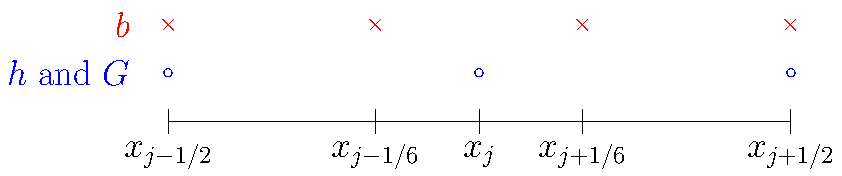
\includegraphics[width=0.8\textwidth]{./Figures/Diagrams/FEMbasis/Reconstruction/FEVMRecon.pdf}
	\caption{The locations of the reconstructions for $h$ and $G$ (\circlet{blue}) and $b$ (\crosst{red}) inside the $j^{th}$ cell.}
	\label{fig:ReconLocs}
\end{figure} 

\subsubsection{The conserved quantities, $h$ and $G$ }
Since $h$ and $G$ use the same reconstruction operators they are demonstrated for a general quantity $q$. The values of $q$ are reconstructed at $x_{j-1/2} $, $x_{j} $ and $x_{j+1/2}$ from the cell averages $\overline{q}_j$ using the generalised minmod limiter \cite{VanLeer-1979-101}
%cite someone 
	\begin{align}
	q^+_{j-1/2} = \overline{q}^n_j - \dfrac{\Delta x}{2} d_j &,&
	q_{j}  =\overline{q}^n_j &,&
	q^-_{j+1/2}  = \overline{q}^n_j + \dfrac{\Delta x}{2} d_j
		\label{eqn:ReconforhwG}
	\end{align}
where 
\begin{equation}
d_j = \text{minmod}\left(\theta \dfrac{\overline{q}^n_j -\overline{q}^n_{j-1} }{\Delta x}, \dfrac{\overline{q}^n_{j+1} -\overline{q}^n_{j-1} }{2\Delta x}, \theta\dfrac{\overline{q}^n_{j+1} -\overline{q}^n_{j} }{\Delta x}\right)
\label{eqn:slopehGrecon}
\end{equation}
with $\theta \in \left[1,2\right]$. Note that although $h$ and $G$ have three reconstruction locations in Figure \ref{fig:ReconLocs}, the resultant reconstructed function is a linear polynomial as the reconstructed nodal value is the average of the cell edge values. 

\subsubsection{Bed profile }
The interpolating cubic polynomial for $b$ over the $j^{th}$ cell 
\begin{equation*}
C_j(x) = c_0 \left(x - x_j\right)^3 + c_1 \left(x - x_j\right)^2 + c_2 \left(x - x_j\right) + c_3
\label{eqn:cubicforbedrecon}
\end{equation*}
passing through the adjacent cell nodal values has the coefficients
\begin{align*}
&c_0 =  \dfrac{-b_{j-2} + 2b_{j-1} - 2 b_{j+1} + b_{j+2}}{12 \Delta x^3}, & &
c_1 =  \dfrac{b_{j-2} - b_{j-1} - b_{j+1} + b_{j+2}}{6 \Delta x^2},\\ \\
&c_2 =  \dfrac{b_{j-2} - 8b_{j-1} + 8 b_{j+1} - b_{j+2}}{12 \Delta x},& &
c_3 =  \dfrac{-b_{j-2}  + 4b_{j-1} + 4 b_{j+1} - b_{j+2}}{6}.
\end{align*}

For the weak form of \eqref{defn:SerreEqnConservedQuantity1} to be valid, the bed profile must be continuous. To force a continuous bed profile the two possible values for $b$ at the cell edges are averaged. Hence the reconstructing cubic for $b$ takes the following values
\begin{align}
\label{eqn:BedReconDef}
b_{j\pm1/2} =  \frac{1}{2}\left( C_j(x_{j\pm 1/2}) + C_{j\pm 1}(x_{j\pm 1/2})\right)&,& 	b_{j\pm 1/6} =  C_j(x_{j\pm 1/6}).
\end{align}
To calculate the derivatives of the bed $\left({\partial {b}}/{\partial x} \right)^\pm_{j + 1/2}$ we use the reconstructed cubic polynomial
\begin{align*}
P^b_j(x) = p^b_0 (x - x_j)^3 + p^b_1(x-x_j)^2 + p^b_2(x- x_j) + p^b_3
\end{align*}
which passes through the values \eqref{eqn:BedReconDef} and therefore has the following coefficients
\begin{align*}
&p^b_0 =  \dfrac{-9b_{j-1/2} + 27b_{j-1/6} - 27 b_{j+1/6} + 9b_{j+1/2}}{2 \Delta x^3}, 
&p^b_1 =  \dfrac{9b_{j-1/2} - 9b_{j-1/6} - 9b_{j+1/6} + 9b_{j+1/2}}{4 \Delta x^2},\\ \\ 
&p^b_2 =  \dfrac{b_{j-1/2} - 27b_{j-1/6} + 27 b_{j+1/6} - b_{j+1/2}}{8 \Delta x},
&p^b_3 =  \dfrac{-b_{j-1/2}  + 9b_{j-1/6} + 9 b_{j+1/6} - b_{j+1/2}}{16}.
\end{align*}
So that the bed derivatives of \eqref{eqn:FluxIrrotNum} are approximated as follows
\begin{align}
\label{eqn:PolyDerivb}
&\left(\dfrac{\partial {b}}{\partial x} \right)^-_{j + 1/2} = \frac{\partial }{\partial x}P^b_j(x_{j+1/2}), 
&\left(\dfrac{\partial {b}}{\partial x} \right)^+_{j + 1/2} = \frac{\partial }{\partial x}P^b_{j+1}(x_{j+1/2}). 
\end{align}

\subsection{Calculating $u$ and $\partial u / \partial x$}
To calculate $u$ and $\partial u / \partial x$ a FEM is used to solve \eqref{defn:SerreEqnConservedQuantity1} for $u$ given $h$, $G$ and $b$. The FEM begins with the weak form of \eqref{defn:SerreEqnConservedQuantity1} using a test function $v$ over the spatial domain $\Omega$ resulting in
\begin{equation*}
\int_{\Omega } G v \; dx =  \int_{\Omega } uh \left(1 + \frac{\partial h}{\partial x}\frac{\partial b}{\partial x} + \frac{1}{2}h\frac{\partial^2 b}{\partial x^2} +  \left[\frac{\partial b}{\partial x}\right]^2 \right) v - \frac{\partial}{\partial x}\left(\frac{1}{3}h^3  \frac{\partial {u}}{\partial x}\right) v \; dx.
\end{equation*}
Integrating by parts with zero Dirichlet boundary conditions gives
\begin{multline}
\int_{\Omega } G v \; dx = \int_{\Omega } uh \left(1 + \left[\frac{\partial b}{\partial x}\right]^2 \right) v \; dx +  \int_{\Omega } \frac{1}{3}h^3  \frac{\partial {u}}{\partial x} \frac{\partial v}{\partial x} \; dx  \\ - 
\int_{\Omega }   \frac{1}{2} u h^2\frac{\partial b}{\partial x}  \frac{\partial v }{\partial x}\; dx - 
\int_{\Omega }   \frac{1}{2}h^2\frac{\partial b}{\partial x}  \frac{\partial u }{\partial x}v \; dx.
\label{eqn:WeakFormDomain}
\end{multline}
By assuming that time is fixed so that all the functions only vary in space, this formulation implies that by ensuring that $G$, $h$, $b$ and $\partial b / \partial x$ have finite integrals over $\Omega$, then $u$ and $\partial u / \partial x$ must have finite integrals as well. To approximate the flux and the source terms \eqref{eqn:FullSerreCon} requires $\partial u / \partial x$ to be well defined and thus have finite integrals. So we will assume that for each time $t$ that $h$ and $G$ are square integrable functions and $b$ is in the Sobolev space $\mathbb{W}^{1,2}(\Omega)$ where $b$ and its first weak derivative are square integrable functions so that $u$ is also a member of $\mathbb{W}^{1,2}(\Omega)$.

To approximate \eqref{eqn:WeakFormDomain} the integration is performed over the cells and then summed together to obtain the equation for the entire domain
\begin{multline}
\label{eq:elementwiseint}
\sum_{j=1}^m \Bigg(  \int_{x_{j-1/2} }^{{x_{j+1/2}}} \Bigg[  \left( uh \left(1 + \left[\frac{\partial b}{\partial x}\right]^2 \right)  - \frac{1}{2}h^2\frac{\partial b}{\partial x}  \frac{\partial u }{\partial x}  -  G \right) v   \\ +  \left(\frac{1}{3}h^3  \frac{\partial {u}}{\partial x}    -     \frac{1}{2} uh^2\frac{\partial b}{\partial x}    \right) \frac{\partial v }{\partial x} \Bigg]dx \Bigg)  = 0
\end{multline}
which holds for all test functions $v$. The next step is to replace the functions for $h$, $G$, $b$, $v$ and $u$ with their corresponding basis function approximations.

For $h$ and $G$ the basis functions $\psi$ are linear inside a cell and zero elsewhere, resulting in approximations that are square integrable, as desired.
For $u$ and $v$ the basis functions $\phi$ which are quadratic inside the cell and continuous across the cell edges are used so that the approximations are in $\mathbb{W}^{1,2}(\Omega)$. The basis functions of $u$ must be quadratics to allow for a second-order approximation to $\partial u / \partial x$ in \eqref{eqn:FluxIrrotNum}. Finally, for $b$ the basis functions $\gamma$ are used, they are cubic polynomials inside the cell and continuous across the cell edges so that the approximation to $b$ is in the appropriate function space. Cubic polynomials are used for $b$ as a second-order approximation to $\partial^2 b / \partial x^2$ is required for the source term in \eqref{eqn:FullSerreCon}. Examples of the basis functions $\psi$, $\phi$ and $\gamma$ for the $j^{th}$ cell are given in Figure \ref{fig:P1DiscBasis}, from which their equations can be derived.

\begin{figure}
	\centering
		\begin{subfigure}{0.6\textwidth}
			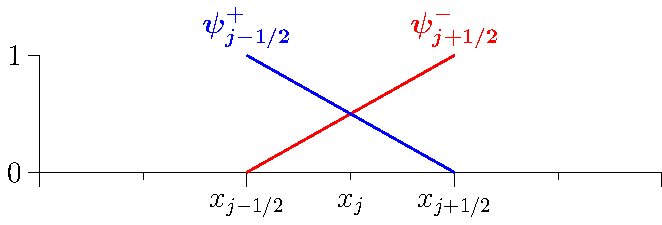
\includegraphics[width=\textwidth]{./Figures/Diagrams/FEMbasis/P1/P1NN-figure0.pdf}
			\subcaption{$\psi$}
			\vspace{0.5cm}
		\end{subfigure}
		\begin{subfigure}{0.6\textwidth}
			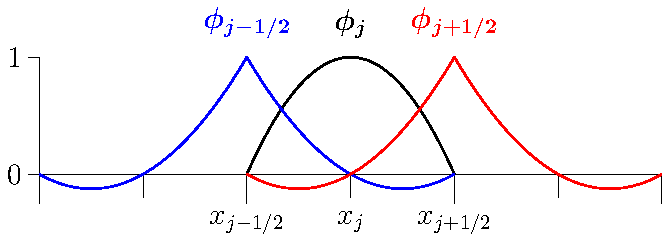
\includegraphics[width=\textwidth]{./Figures/Diagrams/FEMbasis/P2/P2N-figure0.pdf}
			\subcaption{$\phi$}
			\vspace{0.5cm}
		\end{subfigure}
		\begin{subfigure}{0.6\textwidth}
			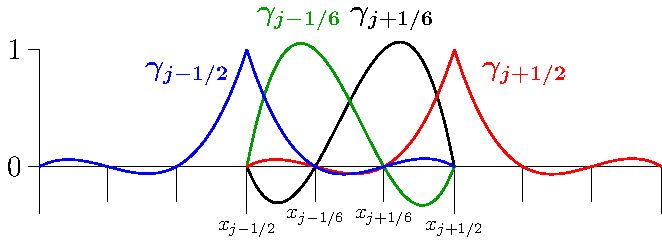
\includegraphics[width=\textwidth]{./Figures/Diagrams/FEMbasis/P3/P3-figure0.pdf}
			\subcaption{$\gamma$}
			\vspace{0.5cm}
		\end{subfigure}
	\caption{Support of the basis functions $\psi$, $\phi$ and $\gamma$ which are non-zero over the $j^{th}$ cell.}
	\label{fig:P1DiscBasis}
\end{figure}

The basis function approximation to $h$ and $G$ in the FEM written for a generic quantity $q$ is
\begin{subequations}
\begin{equation}
\label{eqn:FEapproxtohG}
q = \sum_{j=1}^m \left( q^+_{j-1/2}\psi^+_{j-1/2}  + q^-_{j+1/2}\psi^-_{j+1/2} \right)
\end{equation}
while for $u$ it is
\begin{equation}
u = u_{1/2}\phi_{1/2} + \sum_{j=1}^m \left( u_{j}\phi_{j} + u_{j+1/2}\phi_{j+1/2} \right)
\label{eqn:FEapproxtou}
\end{equation}
and finally for $b$ it is
\begin{equation}
b = b_{1/2}\gamma_{1/2} +  \sum_{j=1}^m \left(b_{j-1/6}\gamma_{j-1/6}  + b_{j+1/6}\gamma_{j+1/6} + b_{j+1/2}\gamma_{j+1/2} \right).
\label{eqn:FEapproxtob}
\end{equation}
\label{eqn:FEapprox}
\end{subequations}
Substituting all the functions in \eqref{eq:elementwiseint} with their corresponding basis function approximations \eqref{eqn:FEapprox} the integral equation becomes a matrix equation. Assembling these matrices results in 
\begin{equation*}
\matr{A} \vecn{\hat{u}} = \vecn{g}.
\end{equation*}
Where $\matr{A}$ is the stiffness matrix given by the integrals that contain $u$, $\vecn{\hat{u}}$ is the vector containing the cell edge and nodal values of $u$ and $\vecn{g}$ is given by the integral of $Gv$. This is a penta-diagonal matrix equation which can be solved by direct banded matrix solution techniques such as those of \citet{NumRecC-1996} to obtain
\begin{equation}
\vecn{\hat{u}} =   \matr{A}^{-1}\vecn{g}
\label{eqn:usolvefromGhb}
\end{equation}
 and thus $u^\pm_{j+1/2}$ is obtained. Note that $u^\pm_{j+1/2} = u_{j+1/2}$ since $u$ is continuous at the cell edges.
 
 To calulate $ \left({\partial {u}}/{\partial x} \right)^\pm_{j + 1/2}$ from $u_{j\pm 1/2}$ and $u_j$ the reconstruction polynomial
\begin{align*}
P^u_j(x) &= p^u_0 (x - x_j)^2 + p^u_1(x-x_j) + p^u_2
\end{align*}
is used. This reconstruction polynomial passes through the values $u_{j\pm 1/2}$ and $u_j$ and so has the following coefficients
\begin{align*}
& p^u_0 =  \dfrac{u_{j-1/2} - 2u_j + u_{j+1/2}}{2 \Delta x^2}, 
& p^u_1 =  \dfrac{-u_{j-1/2} + u_{j+1/2}}{\Delta x},\\
& p^u_2 =  u_j.
\end{align*}
Allowing for the calculations of the derivatives
\begin{align}
&\left(\dfrac{\partial {u}}{\partial x} \right)^-_{j + 1/2} = \frac{\partial }{\partial x}P^u_j(x_{j+1/2}), 
&\left(\dfrac{\partial {u}}{\partial x} \right)^+_{j + 1/2} = \frac{\partial }{\partial x}P^u_{j+1}(x_{j+1/2}).
\label{eqn:PolyDerivu}
\end{align}

\subsection{Source Term Approximation}
To evolve the Serre equations using \eqref{eqn:FVMUpdate} requires an approximation to $S^n_j\left(\vecn{Q}\right)$. Equation \eqref{eqn:FullSerreConMass} has no source term, therefore only the calculation of the source term for equation \eqref{eqn:Serreconsconmom} is presented.

Since \eqref{eqn:FVMUpdate} is temporally first-order accurate the source term approximation
\begin{equation}
S^n_j = -\frac{1}{2}\left(h^n_j\right)^2 {u^n_j}\left( \frac{\partial {u}}{\partial x} \right)^n_j \left(\frac{\partial^2 b}{\partial x^2} \right)^n_j  + h^n_j \left(u^n_j\right)^2 \left(\frac{\partial b}{\partial x}\right)^n_j \left(\frac{\partial^2 b}{\partial x^2}\right)^n_j - gh^n_j\left(\frac{\partial b}{\partial x}\right)^n_j.
\label{eqn:SourceTermNaive}
\end{equation}
is sufficient. The quantities $h^n_j$ and $u^n_j$ are given by \eqref{eqn:ReconforhwG} and \eqref{eqn:usolvefromGhb} respectively. To calculate the derivatives of $b$ and $u$ the approximations outlined in \eqref{eqn:PolyDerivb} and \eqref{eqn:PolyDerivu} respectively are used to obtain
\begin{align*}
\left(\dfrac{\partial {u}}{\partial x} \right)_{j} = \frac{\partial }{\partial x}P^u_j(x_{j})& , &  
\left(\dfrac{\partial {b}}{\partial x} \right)_{j} = \frac{\partial }{\partial x}P^b_j(x_{j})& ,& 	
\left(\dfrac{\partial^2 {b}}{\partial x^2} \right)_{j} = \frac{\partial^2 }{\partial x^2}P^b_j(x_{j}).
\end{align*}

We therefore have all the required approximations to perform the FVM \eqref{eqn:FVMUpdate} and obtain a temporally first-order approximation to \eqref{eqn:FullSerreCon}.

\subsection{Courant-Frederichs-Lewy Condition}
To ensure the stability of the FVM \eqref{eqn:FVMUpdate} the Courant-Friedrichs-Lewy (CFL) condition \cite{Courant-etal-1967-215} is used. The CFL condition is necessary for stability and ensures that time steps are small enough so that information is only transferred between neighbouring cells. For the Serre equations the CFL condition is 
\begin{equation}
\Delta t \le \frac{Cr }{\max_{j} \left\lbrace a^\pm_{j+1/2} \right\rbrace} \Delta x
\label{eqn:CFLcond}
\end{equation}
where $a^\pm_{j+1/2} $ are the wave-speed bounds used in the flux approximation \eqref{eqn:WaveSpeedBoundsFluxApprox} and $0\le Cr \le 1$ is the Courant number. Typically, we use the conservative $Cr = 0.5$ for our numerical experiments.

\subsection{Time-Stepping}
To increase the order of accuracy in time we employ the second-order SSP Runge-Kutta method \cite{Gottlieb-etal-2003-89} which is a convex combination of first-order forward Euler time steps in the following way
\begin{subequations}
	\begin{align}
\overline{\vecn{Q} }^{(1)}_j &= \overline{\vecn{Q} }^{n}_j - \frac{\Delta t}{\Delta x} \left(F^n_{j+1/2}\left(\vecn{Q} \right) - F^n_{j-1/2}\left(\vecn{Q} \right) \right) + \Delta t S^n_j\left(\vecn{Q} \right),\\
\overline{\vecn{Q} }^{(2)}_j &= \overline{\vecn{Q} }^{(1)}_j - \frac{\Delta t}{\Delta x} \left(F^{(1)}_{j+1/2}\left(\vecn{Q} \right) - F^{(1)}_{j-1/2}\left(\vecn{Q} \right) \right) + \Delta t S^{(1)}_j\left(\vecn{Q} \right),\\
	\overline{\vecn{Q} }^{n+1}_j &= \frac{1}{2} \left( \overline{\vecn{Q} }^n_j +  \overline{\vecn{Q} }_j^{(2)}  \right).
	\end{align}
	\label{eqn:SSPRKStep1}
\end{subequations}

This results in a time stepping method that preserves the stability of the first-order method and is second-order accurate in time. Since all the spatial approximations are second-order accurate, the FEVM should be a second-order accurate solver for the Serre equations, as desired. 

\subsection{Well Balancing Modifications}
To ensure that the method is well-balanced the work of \citet{Klein-etal-2004-2050} is followed. This method was originally designed for the SWWE but was shown to apply equally well to the Serre equations \cite{Pitt-J-2014}.

The well balancing approach makes two changes to the method outlined above. The well-balancing introduces a different reconstruction of $h$ replacing the reconstructed $h$ values in the flux terms \eqref{eqn:FluxMassNum} and \eqref{eqn:FluxIrrotNum}. Additionally, correction terms are added to the source term approximation \eqref{eqn:SourceTermNaive}. These changes ensure that the numerical approximations to the hydrostatic pressure term in the flux and the source term cancel for the lake at rest problem.

\subsubsection{Modified Reconstruction of $h$}
The modified reconstruction of $h$, $\ddot{h}$ depends on the reconstructions $w^-_{j+1/2}$ and $w^+_{j+1/2}$ of $w$ at the cell edge, which is calculated from its cell average values in the same way as $h$ and $G$, \eqref{eqn:slopehGrecon}. From these reconstructions the bed values
\begin{align*}
\dot{b}^-_{j+1/2} = w^-_{j+1/2} - h^-_{j+1/2} &, &\dot{b}^+_{j+1/2} = w^+_{j+1/2} - h^+_{j+1/2}
%\label{eqn:BedReDefWmH}
\end{align*}
are calculated. Given the maximum of these bed values
\begin{align*}
\ddot{b}_{j+1/2} = \max\left\lbrace\dot{b}^-_{j+1/2} , \dot{b}^+_{j+1/2} \right\rbrace
\end{align*}
the reconstruction $\ddot{h}$ at the cell edges is given by
\begin{align}
&\ddot{h}^-_{j+1/2} = \max\left\lbrace 0, w^-_{j+1/2} - \ddot{b}_{j+1/2}  \right\rbrace, &\ddot{h}^+_{j+1/2} = \max\left\lbrace 0, w^+_{j+1/2} - \ddot{b}_{j+1/2} \right\rbrace.
\label{eqn:ModifiedHValue}
\end{align}
which replaces $h^\pm_{j+1/2}$ in the flux terms \eqref{eqn:FluxMassNum} and \eqref{eqn:FluxIrrotNum}.

\subsubsection{Modified Source Term}
The source term is modified by adding the corrective interface source terms $S^{-}_{j + \frac{1}{2}}$ and $S^{+}_{j + \frac{1}{2}}$ to obtain
\begin{equation*}
S^n_j =  \frac{1}{\Delta x}S^{-}_{j + \frac{1}{2}} +  S_{ci} +  \frac{1}{\Delta x}S^{+}_{j - \frac{1}{2}}.
\end{equation*}
Where $S_{ci}$ is the source term approximation given in \eqref{eqn:SourceTermNaive} with the approximation to $\partial b / \partial x$ altered to depend on $\dot{b}^-_{j+1/2}$ and $\dot{b}^+_{j-1/2}$ like so
\begin{align*}
\left(\dfrac{\partial {b}}{\partial x} \right)_{j} =  \frac{\dot{b}^-_{j+1/2} - \dot{b}^+_{j-1/2}}{\Delta x}.
\end{align*}

The corrective interface source terms are calculated in the following way
\begin{align*}
S^{-}_{j + \frac{1}{2}} =  \frac{g}{2} \left(\ddot{h}^{-}_{j + \frac{1}{2}} \right)^2 - \frac{g}{2} \left(h^{-}_{j + \frac{1}{2}} \right)^2&,&
S^{+}_{j - \frac{1}{2}} =  \frac{g}{2} \left(h^{+}_{j - \frac{1}{2}}\right)^2 - \frac{g}{2}\left(\ddot{h}^{+}_{j - \frac{1}{2}}\right)^2 .
\end{align*}
These corrective terms make use of $h^{-}_{j + \frac{1}{2}}$ and $h^{+}_{j + \frac{1}{2}}$ obtained from the reconstruction \eqref{eqn:ReconforhwG} and the other reconstructions $\ddot{h}^{-}_{j + \frac{1}{2}}$ and $\ddot{h}^{+}_{j + \frac{1}{2}}$ from \eqref{eqn:ModifiedHValue}. 

\subsection{Dry Bed Handling Modifications}
Dry beds present two issues for the FEM; when $h$ and $G$ are small then small errors in $h$ and $G$ can produce large errors in $u$ leading to instabilities and when $h=0$ the stiffness matrix $\matr{A}$, \eqref{eqn:usolvefromGhb} becomes singular.

The issue of large errors in $u$ when $h$ is small also arises when solving the SWWE; due to $u = (uh)/h $ being undefined as $u h $ and $h$ vanish. For the Serre equations with horizontal beds when $h \ll 1$ from \eqref{defn:SerreEqnConservedQuantity1} we have
\begin{equation*}
G = uh + \mathcal{O}\left(h^3\right).
\end{equation*}
Since $h \ll 1$ the $\mathcal{O}\left(h^3\right)$ terms can be neglected, and thus when $h$ is small $G$ is approximately equal to the momentum $uh$. Hence, the challenges posed by $h \rightarrow 0$ for the SWWE and the Serre equations are similar. Therefore, the dry bed handling techniques from the SWWE can be applied to the Serre equations; in particular a desingularisation transformation \cite{Kurganov-Petrova-2007-707}. 

These desingularisation transforms act by modifying the calculation of $u$ given $h$ and $uh$ to avoid the singularity as the numerator and denominator approach zero, hence their name. The simplest such transformation is
\begin{equation}
u = \frac{(uh) h}{h\left(h + h_{base}\right)}
\label{eqn:calculationofugivenuhandh}
\end{equation}
where $h_{base}$ is some small chosen parameter. The error introduced by this transformation is smallest when $h_{base}$ is smallest. However, as noted by \citet{Kurganov-Petrova-2007-707} small values of $h_{base}$ lead to large numerical errors in the calculation of $u$. To avoid such errors $h_{base}$ can be made larger or following \citet{Kurganov-Petrova-2007-707} different desingularisation transformations can be employed. For the validations described later, we found the simpler transformation with small values of $h_{base}$ more useful, keeping in mind that large numerical errors in $u$ were possible for small values of $h$. 

To adapt the calculation of $u$ in \eqref{eqn:calculationofugivenuhandh} to \eqref{defn:SerreEqnConservedQuantity1} we view it as a transformation of the quantity $h$ which is equivalent to
\begin{equation}
\label{eqn:hsimpletransform}
h \rightarrow h \left( \frac{h + h_{base}}{h} \right).
\end{equation}
This transformation is ill-defined when $h = 0$ so we also add in a small term $h_{tol}$ to the denominator. This $h_{tol}$ also serves as our cut-off value with any cells with $\overline{h}_j < h_{tol}$ considered as dry. Therefore, our transformation for the reconstructed values of $h$ in the finite element method is
\begin{align}
\label{eqn:hdrytransform}
h^+_{j-1/2}  = h^+_{j-1/2} \left(\frac{ h^+_{j-1/2}  + h_{base}}{h^+_{j-1/2} + h_{tol}}\right) &,&
h^-_{j+1/2}  = h^-_{j+1/2} \left(\frac{ h^-_{j+1/2}  + h_{base}}{h^-_{j+1/2} + h_{tol}}\right)
\end{align} 
where on the right hand side are the reconstructed values of $h$ from \eqref{eqn:ReconforhwG} and the left hand side are the values of $h$ used to defined the basis functions of the FEM \eqref{eqn:FEapproxtohG}. This transformation is applied to all terms in the FEM avoiding the singularity in \eqref{eqn:hsimpletransform} as $h \rightarrow 0$.

Even with the transform \eqref{eqn:hdrytransform}, the matrix $\matr{A}$ can become singular. To circumvent this an LU decomposition with partial pivoting \cite{NumRecC-1996} was employed. Typically we set the pivot tolerance value $p_{tol} = 10^{-20}$ allowing the matrix solver to accurately invert $\matr{A}$ in \eqref{eqn:usolvefromGhb} when $h = 0$. 

Finally, to avoid very large errors in $u$ we identify dry cells when the cell average value of $h$ is very small. A cell is considered dry when $\overline{h}_j \le h_{tol}$. For dry cells we set
\begin{align*}
& 	h^+_{j-1/2}  = 0,   & 	G^+_{j-1/2}  = 0, & & 	w^+_{j-1/2}  = b_{j-1/2},   \\
&	h_{j} = 0, & 	G_{j}  = 0,  & 	&w_{j}  = b_{j},\\
& 	h^-_{j+1/2}  = 0,  & 	G^-_{j+1/2}  = 0, & 	&w^-_{j+1/2}  = b_{j+1/2}, \\
& u_j = 0
\end{align*}
and if the neighbouring cells are dry then the velocity at the cell edges vanish so that
\begin{align*}
& 	u_{j-1/2}  = 0  &\text{when}& &\overline{h}_{j-1}\le h_{tol}, \\
& 	u_{j+1/2}  = 0  &\text{when}& &\overline{h}_{j+1} \le h_{tol}.
\end{align*}
The identification of dry cells occurs after the solution of \eqref{eqn:usolvefromGhb}. In the numerical experiments the typical values used were $h_{tol} = 10^{-12}$ and $h_{base} = 10^{-8}$.

%----------
\section{Validation}
To validate that the numerical method is the appropriate order of accuracy, well-balanced and can handle dry-beds we used an analytic solution, forced solution and experimental results. Firstly, the convergence and conservation properties of the method for the lake at rest analytic solution were measured. Secondly, we measured the convergence of the numerical method to a forced solution of the Serre equations. Finally, we compared our numerical solutions to the experimental results of \citet{Synolakis-1987-523}.


\subsection{Measures of Convergence and Conservation}
We begin the validation by defining the measures of convergence and conservation for a general quantity $q$. The $L_2$ vector norm was used to measure the difference between a numerical solution at the cell nodes $\vecn{q^*}$ and the analytic or forced solution at the cell nodes $\vecn{q}$ using
\begin{equation*}
L_2(\vecn{q},\vecn{q^*}) =  \left\lbrace \begin{array}{c r} 
\dfrac{||\vecn{q^*} - \vecn{q}||_{2}}{||\vecn{q}||_{2}} & ||\vecn{q}||_{2} > 0 \\ \\
{||\vecn{q^*}||_{2}} & ||\vecn{q}||_{2} = 0 . \end{array}\right. 
\label{eqn:L1qdef} 
\end{equation*} 
By investigating the behaviour of $L_2(\vecn{q},\vecn{q^*})$ for numerical solutions with various $\Delta x$ values we can establish the convergence rate of the method. 

The conservation properties of the method are studied using the conservation error $C^*$. The conservation error $C^*$ compares the total amount of $q$ in the numerical solution at the end of the simulation $\mathcal{C}^*\left({\vecn{q^*}}\right)$ to the total amount of $q$ in the initial conditions $\mathcal{C}^*\left({\vecn{q}}\right)$ as follows
\begin{equation*}
C^*(\vecn{q},\vecn{q^*}) =  \left\lbrace \begin{array}{c r} 
\dfrac{|\mathcal{C}^*\left({\vecn{q^*}}\right) - \mathcal{C}^*\left({\vecn{q}}\right)| }{|\mathcal{C}^*\left({\vecn{q}}\right)|} & |\mathcal{C}^*\left({\vecn{q}}\right)| > 0 \\ \\
|\mathcal{C}^*\left({\vecn{q^*}}\right)| & |\mathcal{C}^*\left({\vecn{q}}\right)| = 0  . \end{array}\right. 
\end{equation*}
Where the total amount of a quantity $\mathcal{C}^*\left({\vecn{q}}\right)$ is calculated numerically by summing the total amount of $q$ in each cell.
With fifth-order accurate Gaussian quadrature of a quartic interpolation of $q$ using the neighbouring nodal values used to calculate the total amount of $q$ in a cell.
\subsection{Lake at Rest Solution Validation}
The lake at rest is a stationary analytic solution of the Serre equations where a still lake has a horizontal water surface over any bathymetry. This solution is maintained due to the balance of the hydrostatic pressure and the forcing of the bed slope. A well-balanced numerical method should accurately reproduce this lake at rest stationary solution.

To test whether this method is well-balanced we chose the following lake at rest solution
	\begin{align*}
	&h(x,t) = \max\left\lbrace a_0 - b(x), 0 \right\rbrace, & b(x) = a_1 \sin\left(a_2 x\right), \\
	&u(x,t) = 0 , 	&G(x,t) = 0.
	\end{align*}
To demonstrate the capability of the method in the presence of dry and wet beds the parameter values $a_0 = 0m$, $a_1 = 1m$ and $a_2 = 2 \pi / 50 m^{-1} $ were chosen. These parameter values result in lakes with a horizontal free surface surrounded by dry regions.

For the numerical solutions the spatial domain was $x \in \left[-112.5 m,87.5 m\right]$ and the final time was $t=10s$, with the standard gravitational acceleration $g= 9.81 m/s^2$. The spatial resolution of the method was varied so that $\Delta x = 100 / 2^k m$ with $k \in \left[8, \dots ,17\right]$ and the CFL condition \eqref{eqn:CFLcond} was satisfied by having $\Delta t = Cr \Delta x / \sqrt{g}$ with condition number $Cr = 0.5$. The standard limiter parameter $\theta = 1.2$ was used in the generalised minmod limiter \eqref{eqn:slopehGrecon}. Dirichlet boundary conditions were used at both ends as the analytic solution is stationary.

The numerical method is assessed by using the specified lake at rest solution as initial conditions and comparing the numerical solution at $t=10s$ to the analytic solution, which are the initial conditions.

An example numerical solution with $\Delta x = 100/2^{10}m \approx 0.0977m$ at $t=10s$ is given in Figure \ref{fig:LAR}. The numerical solution in this figure is indistinguishable from the analytic solution at this scale and so the analytic solution has been omitted. 

\begin{figure}
	\centering
		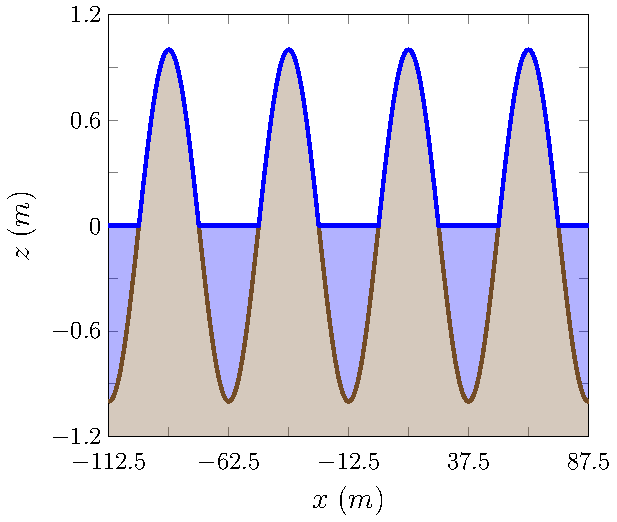
\includegraphics[width=0.5\textwidth]{./Figures/LakeAtRest/Exw.pdf}
	\caption{Numerical solution for $w$ (\squareF{blue}) and $b$ (\squareF{brown!60!black}) with $\Delta x = {100} / {2^{10}}m $ for the lake at rest problem at $t=10s$.}
	\label{fig:LAR}
\end{figure}
\begin{figure}
	\centering
	\begin{subfigure}{0.49\textwidth}
		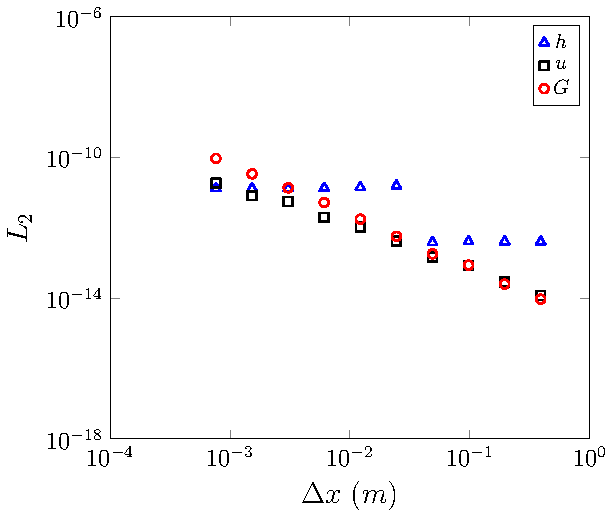
\includegraphics[width=\textwidth]{./Figures/LakeAtRest/L2.pdf}
		\subcaption{Convergence ($L_2$)}
		\label{fig:LARL1}
		\vspace{0.5cm}
	\end{subfigure}
	\begin{subfigure}{0.49\textwidth}
		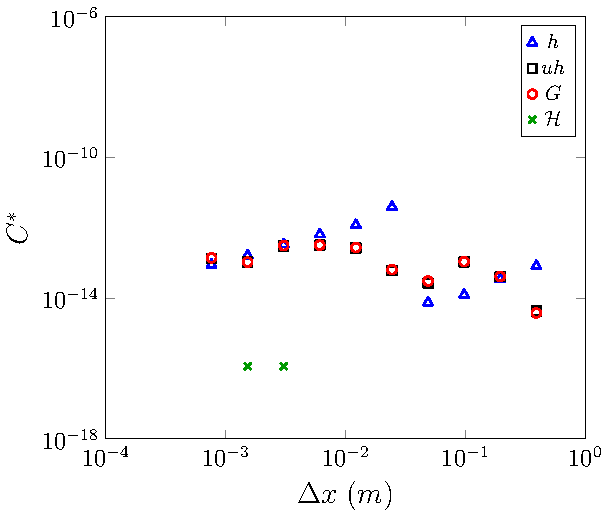
\includegraphics[width=\textwidth]{./Figures/LakeAtRest/C1num.pdf}
		\subcaption{Conservation Error ($C^*$)}
		\label{fig:LARC}
		\vspace{0.5cm}
	\end{subfigure}
	\caption{Convergence ($h$, $u$ and $G$) and conservation error ($h$, $uh$, $G$ $\mathcal{H}$) against $\Delta x$ for the lake at rest problem at $t=10s$. }
	\label{fig:LARL2C}
\end{figure}

Examination of the $L_2$ errors depicted in Figure \ref{fig:LARL2C}(a) reveals that the method reproduced $h$, $G$ and $u$ precisely, accounting for round-off errors. For $h$, $G$ and $u$ their errors are increasing as $\Delta x \rightarrow 0$ due to an accumulation of the round-off errors. 

The conservation errors as measured by $C^*$ for $h$, $uh$, $G$ and $\mathcal{H}$ are given in Figure \ref{fig:LARL2C}(b). The conservation error of these conserved quantities demonstrates that all quantities are conserved within machine precision. With $\mathcal{H}$ being conserved exactly for most numerical solutions, hence its disappearance from the log-log plot. The conservation error of $\mathcal{H}$ is small for the lake at rest solution since $u$ and therefore the kinetic energy is very small. 

These results demonstrate that the developed method has accurately reproduced the lake at rest solution and is therefore well-balanced.

%--------------------------------------------------------------------------------
\subsection{Forced Solution Validation}
There are currently no known analytic solution of the Serre equations for the wetting and drying of varying bathymetry. To test the capability of our numerical method in this environment we resort to a forced solution.

To force a solution we select some arbitrary function for all of the primitive quantities; $h$, $u$ and $b$ which we denote by $h^\#$, $u^\#$ and $b^\#$ respectively. To ensure that these functions $h^\#$, $u^\#$ and $b^\#$ are exact solutions the Serre equations are modified by adding the terms $S_{h} $ and $S_{G}$ to obtain the forced Serre equations
\begin{align*}
& \frac{\partial h}{\partial t} + \dfrac{\partial (uh)}{\partial x} + S_{h}  = 0 ,  \\ \nonumber \\
\begin{split}
\frac{\partial G}{\partial t}  + \frac{\partial}{\partial x} \left( {u} G + \frac{gh^2}{2} - \frac{2h^3}{3} \left[ \frac{\partial {u}}{\partial x} \right]^2 + h^2 {u}\frac{\partial {u}}{\partial x}\frac{\partial b}{\partial x} \right) \\ \\ + \frac{uh^2 }{2}\frac{\partial {u}}{\partial x} \frac{\partial^2 b}{\partial x^2}  - h {u}^2\frac{\partial b}{\partial x}\frac{\partial^2 b}{\partial x^2} + gh\frac{\partial b}{\partial x} + S_{G} = 0
\end{split}
\end{align*}
where
\begin{align*}
&  S_{h} = -\frac{\partial h^\#}{\partial t} - \dfrac{\partial (u^\#h^\#)}{\partial x} ,  \\ \nonumber \\
\begin{split}
S_{G} = -\frac{\partial G^\#}{\partial t}  - \frac{\partial}{\partial x} \left( {u}^\# G^\# + \frac{g\left[h^\#\right]^2}{2} - \frac{2\left[h^\#\right]^3}{3} \left[\frac{\partial {u}^\#}{\partial x}\right]^2 + \left[h^\#\right]^2 {u^\#}\frac{\partial {u}^\#}{\partial x}\frac{\partial b^\#}{\partial x} \right) \\ \\ - \frac{{u}^\#\left[h^\#\right]^2 }{2} \frac{\partial {u}^\#}{\partial x} \frac{\partial^2 b^\#}{\partial x^2}  + h^\# {\left[u^\#\right]}^2\frac{\partial b^\#}{\partial x}\frac{\partial^2 b^\#}{\partial x^2} - gh^\#\frac{\partial b^\#}{\partial x}.
\end{split}
\end{align*} 
These forced Serre equations are then numerically solved by solving the Serre equations \eqref{eqn:FullSerreCon} with the analytic values of $S_{h}$ and $S_{G}$ given $h^\#$, $u^\#$ and $b^\#$. So that, the only error present in the numerical solutions of the forced Serre equations is the error produced by the numerical method used to solve the Serre equations.

Note that since the choice of the forced solutions $h^\#$, $u^\#$ and $b^\#$ is arbitrary the solutions of the forced Serre equations need not be conservative or retain any properties of the underlying Serre equations. 

\subsubsection{Dry Bed Forced Solution Problem}
To test the capability of the numerical method to solve the Serre equations the following forced solutions
\begin{subequations}
	\begin{align}
	\label{eqn:ForcedSolutionxt}
	h^\#(x,t) &=  a_0 \exp\left(-\dfrac{\left[\left(x - a_1 t\right) - a_2\right]^2}{2 a_3}\right), \\
	u^\#(x,t) &= a_4 \exp\left(-\dfrac{\left[\left(x - a_1 t\right) - a_2\right]^2}{2 a_3}\right), \\
	b^\#(x) &= a_5 \sin\left(a_6 x\right)
	\end{align}
\end{subequations}
for the primitive variables was chosen. These functions produce a Gaussian bump for $h$ and $u$ that travels at a fixed speed $a_1$ over a dry periodic bed. Thus, $h$ and $u$ will have constant shape and travel to the right over time. However, this is not the case for $G$ because of its dependence on the bed slope which varies over $x$.

The values $a_0 = 0.5m$, $a_1 = 2 \pi / \left(10 a_7\right) m/s$, $a_2 =- 3\pi/ \left(2 a_6\right)m$, $a_3 = \pi / (16 a_6) m^2$, $a_4 = 0.5 m/s$, $a_5 = 1.0 m$ and $a_6 = \pi / 25 m^{-1}$ were used. These parameter values result in a Gaussian bump in $h$ and $u$ that has a width much smaller than the wavelength of the bed profile and travels precisely one wavelength of the bed in $10s$. 

The domain of the numerical solutions was $x \in \left[-112.5 m,87.5 m\right]$ with $t \in \left[0s,10s\right]$. The standard gravitational acceleration $g= 9.81 m/s^2$ was used. The spatial resolution of numerical methods was varied like so $\Delta x = 100 / 2^k m$ with $k \in \left[8,\dots,17\right]$. To satisfy the CFL condition \eqref{eqn:CFLcond} the temporal resolution
$\Delta t = Cr \Delta x / \left(a_1 + a_4 + \sqrt{g\left(a_0\right)}\right)$ was chosen with condition number $Cr = 0.5$. The value $\theta = 1.2$ was used in the generalised minmod limiter \eqref{eqn:slopehGrecon} and Dirichlet boundary conditions were applied at the boundaries of the domain. 
\begin{figure}
	\centering
	\begin{subfigure}{0.5\textwidth}
		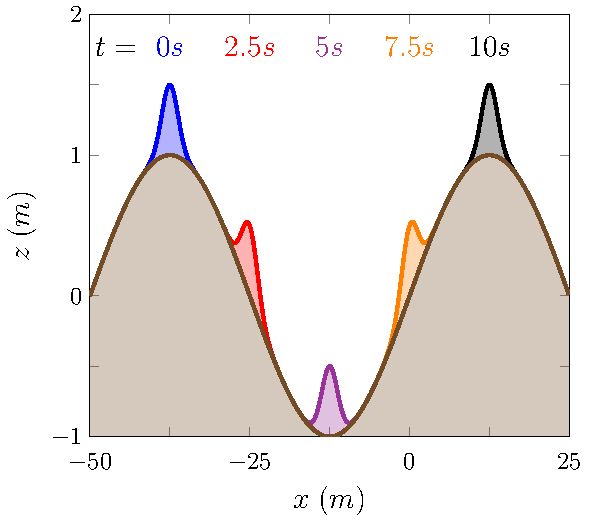
\includegraphics[width=\textwidth]{./Figures/Forced/Dry/w.pdf}
		\subcaption{$w$ and $b$ (\squareF{brown!60!black})}
		\vspace{0.2cm}
	\end{subfigure}%
	\begin{subfigure}{0.5\textwidth}
	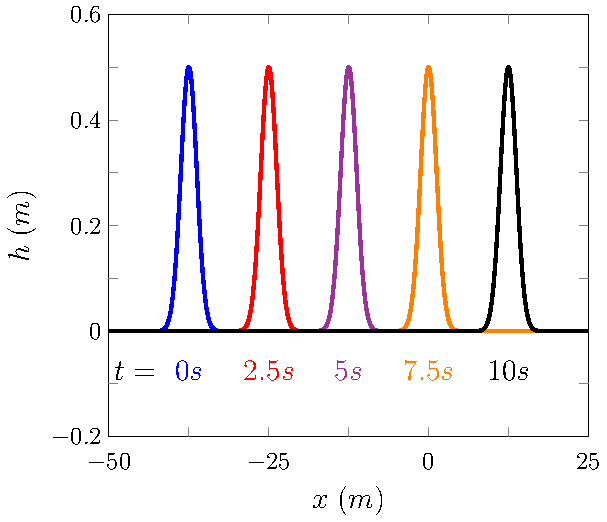
\includegraphics[width=\textwidth]{./Figures/Forced/Dry/h.pdf}
		\subcaption{$h$}
		\vspace{0.2cm}
	\end{subfigure}
	\begin{subfigure}{0.5\textwidth}
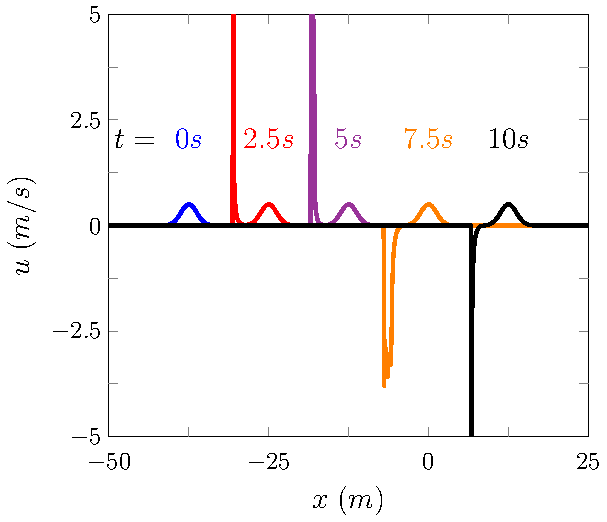
\includegraphics[width=\textwidth]{./Figures/Forced/Dry/u.pdf}
\subcaption{$u$}
		\vspace{0.2cm}
	\end{subfigure}%
	\begin{subfigure}{0.5\textwidth}
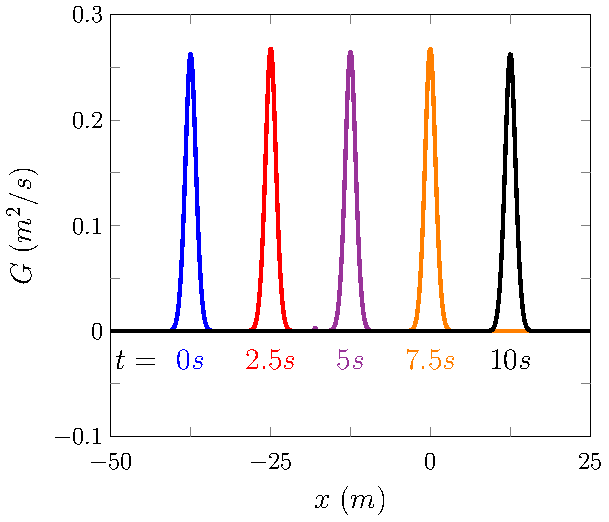
\includegraphics[width=\textwidth]{./Figures/Forced/Dry/G.pdf}
\subcaption{$G$}
		\vspace{0.2cm}
	\end{subfigure}
	\caption{Example numerical solutions for $w$, $b$, $h$, $G$ with $\Delta x = 100 / 2^{10}m$ at various times to the dry bed forced solution problem.}
	\label{fig:ExampleForcedSolutionDry}
\end{figure}
\begin{figure}
	\centering
		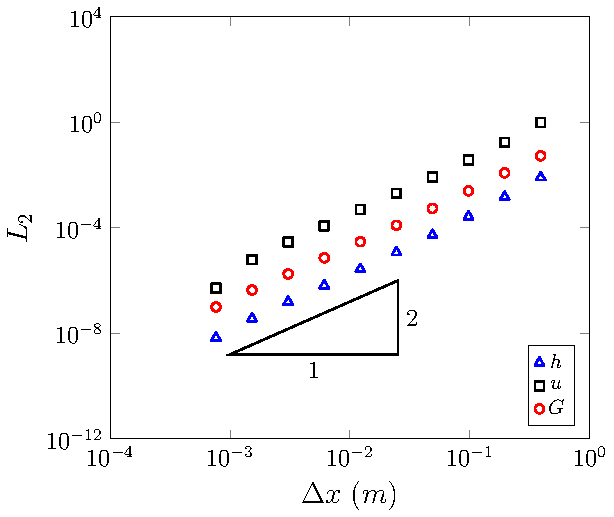
\includegraphics[width=0.5\textwidth]{./Figures/Forced/Dry/L2red.pdf}
	\caption{Convergence as measured by the $L_2$ in regions where $h > 10^{-3}m$ against $\Delta x$ for $h$, $u$, and $G$ for the dry bed forced solution problem at $t=10s$.}
	\label{fig:L1convergenceforcedWet}
\end{figure}
%[]

Plots of $w$, $h$, $u$ and $G$ are given in Figure \ref{fig:ExampleForcedSolutionDry} for the numerical solution with $\Delta x = 100 / 2^{10}m\approx 0.0977m$. The numerical solutions of $w$, $h$ and $G$ well reproduce their respective forced solutions. However, $u$ contains large errors behind the Gaussian bump which are caused by the particular choices $h_{{base}} = 10^{-8}$ and $h_{{tol}} = 10^{-12}$ used in the desingularisation transformation applied to the FEM, \eqref{eqn:usolvefromGhb}. By choosing larger values for these quantities the errors in $u$ can be significantly damped. However, if $h_{{base}}$ and $h_{{tol}}$ are larger they begin to dominate the $L_2$ errors in $h$ and $G$ making the convergence rate of the method less obvious. This trade-off is present in all desingularisation transforms. 

The goal of using this forced solution was to confirm the convergence rate of the numerical method for the wetting and drying of variables beds. For this purpose the chosen desingularisation transform \eqref{eqn:hdrytransform} with small $h_{{base}}$ and $h_{{tol}}$ values was sufficient, resulting in large observed errors in $u$ when $h$ is small.

%h > 10**-3 lowest
The $L_2$ errors for $h$, $u$ and $G$ in regions where $h > 10^{-3} m$ are given in Figure \ref{fig:L1convergenceforcedWet}. For these regions where $h$ is large the second-order convergence of all quantities is observed. When $h$ is small, the second-order accuracy in the approximation of $u$ is lost but the other quantities retain their second-order convergence as all flux and source terms depend on $u$ multiplied by some power of $h$. Therefore, the large errors in $u$ do not pollute the numerical approximations to the other quantities.


Therefore, this method retains second-order convergence for $h$ and $G$ in the presence of dry beds, even with small $h_{{base}}$ and $h_{{tol}}$ values. Although, in such cases the velocity may have large errors in regions where $h$ is small. For physical applications where large errors in $u$ when $h$ is small are not acceptable we recommend altering the dry bed handling of the scheme by increasing the $h_{{base}}$ and $h_{{tol}}$ values or altering the desingularisation transformation \cite{Kurganov-Petrova-2007-707}. 


%--------------------------------------------------------------------------------
\subsection{Run-up of a Solitary Wave}

To study the run-up of incoming waves on linear beaches a series of experiments were conducted by \citet{Synolakis-1987-523}. These experiments consisted of a number of run-up events for a wide array of breaking and non-breaking waves where snapshots of the entire water surface were taken at certain times. These experiments were all performed on the beach profile depicted in Figure \ref{fig:SynolakisWT}, where all the quantities are non-dimensionalised \cite{Synolakis-1987-523}. To denote that a quantity is non-dimensionalised we use a prime. To assess the numerical method we recreated one of these experiments, which captured the run-up of a non-breaking solitary wave.

The numerical method used the non-dimensionalised quantities reported by \citet{Synolakis-1987-523} to reproduce the experiment. The spatial domain was $x' \in [-30,150]$ with a resolution of $\Delta x = 0.05$ and was run until $t' = 250$ with the CFL condition \eqref{eqn:CFLcond} satisfied by setting $\Delta t = 0.1 \Delta x$. The spatial reconstruction used $\theta = 1.2$ and the acceleration due to gravity $g= 1$ was chosen to match the non-dimensionalisation.

The same initial conditions are used to generate this numerical experiment as those of \citet{Li-2014-169}. This was a leftward travelling solitary wave analytic solution of the Serre equations centred around $x' = 38.5$. Figure \ref{fig:SynolakisWT} demonstrates the initial water surface profile given by these initial conditions. 

The non-dimensionalised water surface data is given at the various times in Figure \ref{fig:SynolakisFEVMNoBreak}. The error in conservation of $h'$, $u'h'$, $G'$ and $\mathcal{H}'$ by $t' = 250$ as measured by $C^*$ are given in Table \ref{tab:ConservationSynFEVM}. 

\begin{figure}
	\centering
	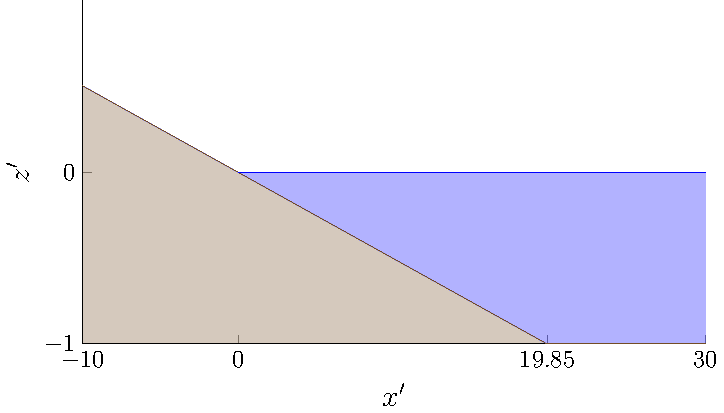
\includegraphics[width=0.5\textwidth]{./Figures/Diagrams/WaveTankSynolakis/WavetankArtifical.pdf}
	\caption{Diagram showing a longitudinal section of the wave tank for the run-up experiment with the water (\squareF{blue}) and the bed (\squareF{brown!80!black}) where the coordinates have been non-dimensionalised \cite{Synolakis-1987-523}.}
	\label{fig:SynolakisWT}
\end{figure}
\begin{figure}
	\centering
	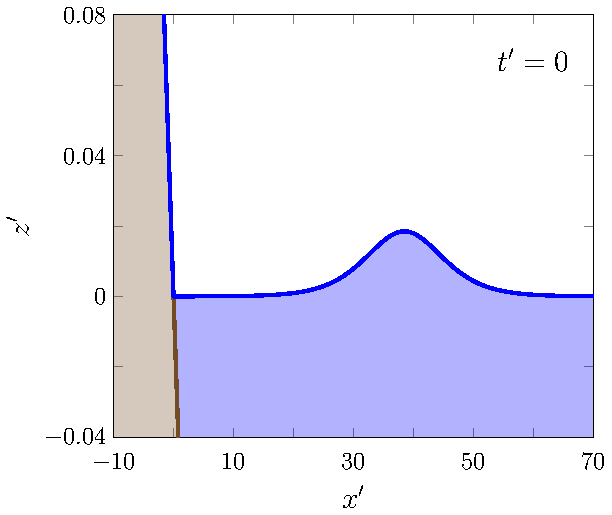
\includegraphics[width=0.5\textwidth]{./Figures/Experimental/Synolakis/nonbreaking/0s.pdf}
	\caption{ Initial water surface profile (\squareF{blue}) over the bed (\squareF{brown!80!black}) for the run-up experiment of \citet{Synolakis-1987-523}.}
	\label{fig:SynolakisInit}
\end{figure}
\begin{figure}
	\centering
	\begin{subfigure}{0.5\textwidth}
		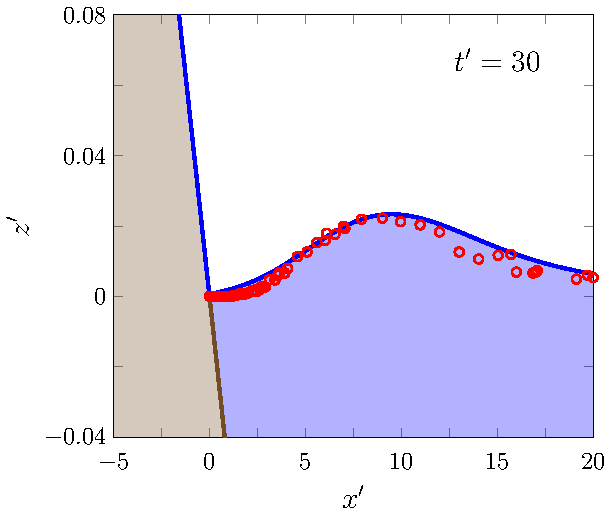
\includegraphics[width=\textwidth]{./Figures/Experimental/Synolakis/nonbreaking/30s.pdf}
		\vspace{0.2cm}
	\end{subfigure}%
	\begin{subfigure}{0.5\textwidth}
		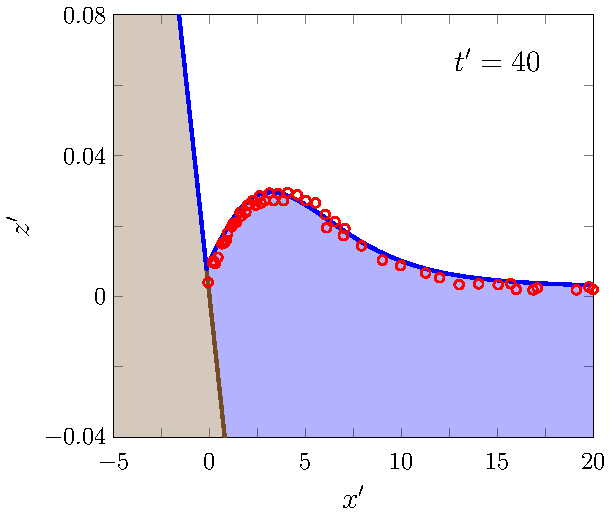
\includegraphics[width=\textwidth]{./Figures/Experimental/Synolakis/nonbreaking/40s.pdf}
		\vspace{0.2cm}
	\end{subfigure}
	\begin{subfigure}{0.5\textwidth}
		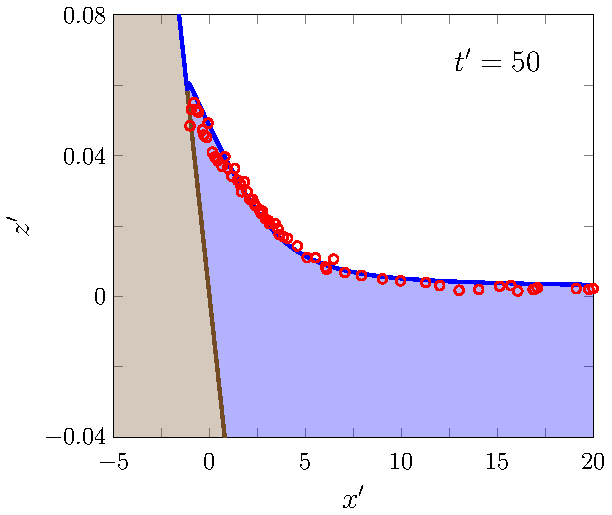
\includegraphics[width=\textwidth]{./Figures/Experimental/Synolakis/nonbreaking/50s.pdf}
		\vspace{0.2cm}
	\end{subfigure}%
	\begin{subfigure}{0.5\textwidth}
		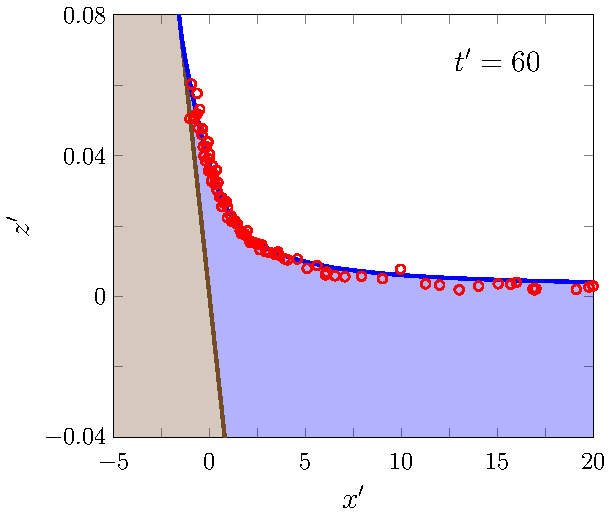
\includegraphics[width=\textwidth]{./Figures/Experimental/Synolakis/nonbreaking/60s.pdf}
		\vspace{0.2cm}
	\end{subfigure}
	\begin{subfigure}{0.5\textwidth}
		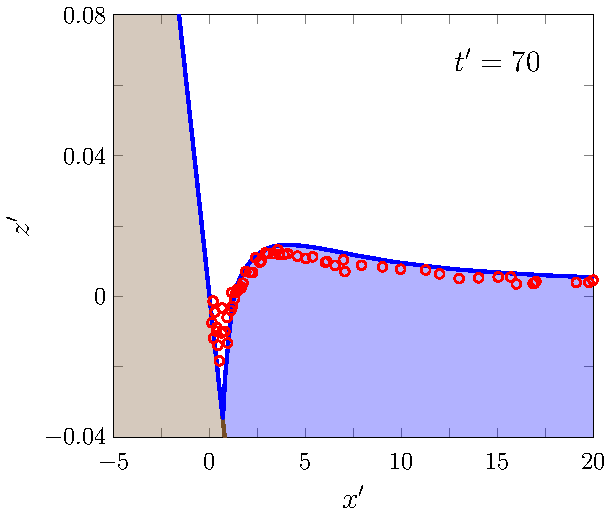
\includegraphics[width=\textwidth]{./Figures/Experimental/Synolakis/nonbreaking/70s.pdf}
		\vspace{0.2cm}
	\end{subfigure}
	\caption{A comparison of the water surface profiles $w'(x',t')$ for the experiment (\circlet{red}) and the numerical solution (\squareF{blue}) over the bed (\squareF{brown!60!black}) at various times.}
	\label{fig:SynolakisFEVMNoBreak}
\end{figure}

The numerical solution reproduces the incoming wave properties and the maximum run-up well, and compares well to numerical solutions presented in the literature \cite{Li-2014-169,Filippini-etal-2016-381}. The experimental wave appears to be more skewed towards the shoreline, but this shape difference has all but disappeared as the wave begins to inundate the shore. The only other noticeable difference is that the numerical solution appears to receed further than the experimental results. The observed larger run-down is likely caused by the omission of bed friction for the Serre equations in this paper.


\begin{table}
	\centering
	\begin{tabular}{l  c  c c}
		Quantity& $\mathcal{C}^*\left(\vecn{q}^0\right)$ & $\mathcal{C}^*\left(\vecn{q}^*\right)$ & ${C}^*\left(\vecn{q}^0,\vecn{q}^*\right)$  \B\\
		\hline 
		$h'$ & $240.416965344$ & $240.416965376$ & $1.33\times 10^{-10}$ \T \\
		$u'h'$ & $-0.319050138516$ & $0.318891991793$ & $4.96\times 10^{-4}$\\
		$G'$ & $-0.319073723126$ & $0.318886191223$ & $5.88\times 10^{-4}$\\
		$\mathcal{H}'$ & $-118.389958187$ & $-118.3900028$ & $3.77 \times 10^{-7}$ \B\\
		\hline \\
	\end{tabular}
	\caption{Initial and final ($t'=250$) total amounts and the conservation error for the conserved quantities in the numerical solution of the run-up experiment. Here the absolute value of the total amount of $uh$ and $G$ are taken in the error as the wave is reflected off the beach.}
	\label{tab:ConservationSynFEVM}
\end{table}

Both $h'$ and $\mathcal{H}'$ are well conserved by the method throughout the run-up and run-down of the wave, particularly $h'$. The total energy $\mathcal{H}'$ of the method is also well conserved, however $\mathcal{H}'$ appears to have slightly increased in the method during the run-up process due to the methods handling of the dry bed problem. During this experiment kinetic energy is converted into gravitational potential energy and then back again as the wave is reflected. By $t' = 250$ the reflection of the wave is complete and so we can see that the total amount of $u'h'$ and $G'$ have changed signs, although their errors are small if this is considered. Given that kinetic energy and gravitational energy were exchanged and the handling of the dry bed, the conservation error of $u'h'$ and $G'$ is good. 

The Serre equations have reproduced the experimental result of \citet{Synolakis-1987-523} very well. Experimentally validating the numerical methods ability to solve the Serre equations for flows over dry beds.

\section{Conclusion}
A second-order numerical method for the one-dimensional Serre equations with varying bathymetry was described. The method uses a FVM to solve the Serre equations in conservation law form and improves previous versions of the FVM solvers for the Serre equations \cite{Zoppou-etal-2017}, by using a FEM to solve for the depth-averaged horizontal velocity. The method is modified to ensure that it is well-balanced, maintaining a steady state solution over an arbitrary bathymetry and able to handle flows over dry beds. The numerical method was validated against the lake at rest stationary solution and shown to be well-balanced. Furthermore, it reproduced forced solutions containing the wetting and drying of variable beds with second-order accuracy, affirming its ability to adequately solve the Serre equations for flows over dry beds. Finally, a numerical solution was compared to the experimental results of \citet{Synolakis-1987-523}, demonstrating the ability of the numerical method to accurately reproduce physical results involving wave run-up on a dry bed. These validation results extend those produced by other solvers of the Serre equations for flows over dry beds
\cite{Tissier-2011,Li-2014-169,Filippini-etal-2016-381,DoCarmo-2019-125} by demonstrating convergence for forced solutions.


\section*{References}
%--------------------------------------------------------------------------------
\bibliographystyle{elsarticle-num-names}
\bibliography{DryBed}
%--------------------------------------------------------------------------------
\end{document}